\subsection{Rectifier Circuit}
The rectifier circuit in Figure~\ref{fig:bridgeSchem} was tested in three
configurations: once with no filter capacitor, once with a~\SI{1}{\micro\farad}
capacitor, and once with a~\SI{100}{\micro\farad}.  Additionally, the
peak-to-peak voltage, average voltage, and minimum voltage were measured using
an oscilloscope in each configuration, a screenshot of which is shown in
Figure~\ref{fig:rectShots}.
%
\begin{figure}[H]
	\centering
	\subfloat[No capacitor]{\label{fig:noCapShot}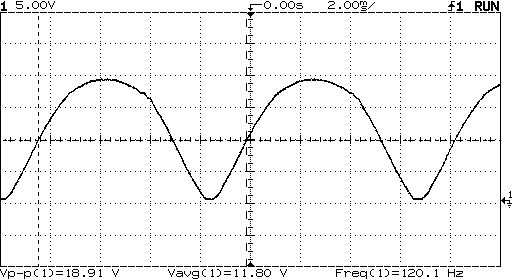
\includegraphics[width=.3\textwidth]{img/shot/bridgeRectNoC.png}}
	\quad
	\subfloat[\SI{1}{\micro\farad} capacitor]{\label{fig:1uFCapShot}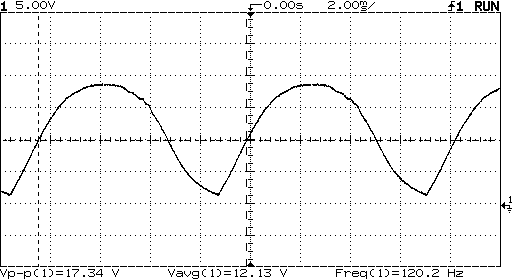
\includegraphics[width=.3\textwidth]{img/shot/bridgeRect1uF.png}}
	\quad
	\subfloat[\SI{100}{\micro\farad} capacitor]{\label{fig:100uFCapShot}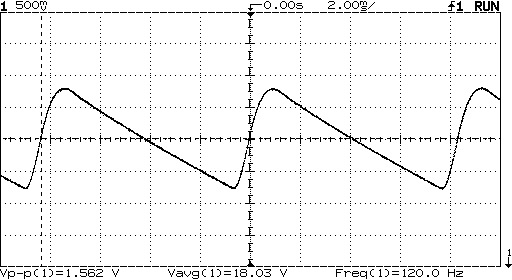
\includegraphics[width=.3\textwidth]{img/shot/bridgeRect100uF.png}}

	\parbox{.9\textwidth}{
	\caption[Oscilloscope Screenshot --- Rectifier Circuit]{Various outputs of
	the rectifier circuit shown in Figure~\ref{fig:bridgeSchem}.  Note that the
	vertical scale in image~\subref{fig:100uFCapShot} is~\SI{.5}{\volt\per
	div}, while the others are~\SI{5}{\volt\per div}.}
	\label{fig:rectShots}}
\end{figure}
%
Data measured by the oscilloscope matches almost exactly the output expected
from the bridge rectifier shown in Figures~\ref{fig:bridgeRectOut}
and~\ref{fig:bridgeRectOutFilt}.  As the size of the filtering capacitor
increases, the output variation decreases.  For each rectifier circuit, the minimum, average, and maximum
values of each waveform were recorded and tabulated into
table~\ref{tab:rectData}.
%
\begin{table}[H]
	\centering
	\begin{tabular}{|c|c|c|c|}
	\hline
	\tbf{Capacitor (\si{\micro\farad}} &
		$\mathbf{V_{p-p}}$ \tbf{(\si{\volt})}&
			$\mathbf{V_{avg}}$ \tbf{(\si{\volt})}&
				$\mathbf{V_{min}}$ \tbf{(\si{\volt})} \\ \hline

	0         & 18.91	& 11.80 	& 0.0  \\ \hline
	1         & 17.34   & 12.13		& 1.6  \\ \hline
    100       & 1.56	& 18.03     & 17.2 \\ \hline
\end{tabular}

	\parbox{.6\textwidth}{
	\caption[Rectifier data]{Tabulated data from the experiments on the bridge
	rectifier.  Note the sharp decrease in peak-to-peak voltage introduced by
	the filtering capacitor.}
	\label{tab:rectData}
	}
\end{table}
%
The recorded values match what is expected of these circuits: as the capacitor
value increases, peak-to-peak voltage decreases sharply, the average value
increases, and the minimum value greatly increases (as a result of the previous
two changes).



Once this procedure has been completed,
a~\SI{2.2}{\kilo\ohm} resistor was placed in parallel with both~$R_1$ and~$R_2$
to for an adequate load.  The source voltage was subsequently swept from~6
to~\SI{30}{\volt} in order to test the line regulation of the IC, or the amount
of change in output per change in input.  Simlarly, the load regulation (change
in output per change in load) of the IC was tested by using a
static~\SI{18}{\volt} source and replacing the load resistor for a decade box.
This resistance was varied from~\SI{100}{\ohm} to~\SI{3.2}{\kilo\ohm}.

\begin{figure}[H]
	\centering
	\begin{tikzpicture}[gnuplot]
%% generated with GNUPLOT 4.4p2 (Lua 5.1.4; terminal rev. 97, script rev. 96a)
%% Fri 14 Oct 2011 11:40:11 AM EDT
\gpsolidlines
\gpcolor{gp lt color axes}
\gpsetlinetype{gp lt axes}
\gpsetlinewidth{1.00}
\draw[gp path] (1.136,0.985)--(10.242,0.985);
\gpcolor{gp lt color border}
\gpsetlinetype{gp lt border}
\draw[gp path] (1.136,0.985)--(1.316,0.985);
\node[gp node right] at (0.952,0.985) { 0};
\gpcolor{gp lt color axes}
\gpsetlinetype{gp lt axes}
\draw[gp path] (1.136,1.433)--(10.242,1.433);
\gpcolor{gp lt color border}
\gpsetlinetype{gp lt border}
\draw[gp path] (1.136,1.433)--(1.316,1.433);
\node[gp node right] at (0.952,1.433) { 1};
\gpcolor{gp lt color axes}
\gpsetlinetype{gp lt axes}
\draw[gp path] (1.136,1.880)--(10.242,1.880);
\gpcolor{gp lt color border}
\gpsetlinetype{gp lt border}
\draw[gp path] (1.136,1.880)--(1.316,1.880);
\node[gp node right] at (0.952,1.880) { 2};
\gpcolor{gp lt color axes}
\gpsetlinetype{gp lt axes}
\draw[gp path] (1.136,2.328)--(10.242,2.328);
\gpcolor{gp lt color border}
\gpsetlinetype{gp lt border}
\draw[gp path] (1.136,2.328)--(1.316,2.328);
\node[gp node right] at (0.952,2.328) { 3};
\gpcolor{gp lt color axes}
\gpsetlinetype{gp lt axes}
\draw[gp path] (1.136,2.776)--(10.242,2.776);
\gpcolor{gp lt color border}
\gpsetlinetype{gp lt border}
\draw[gp path] (1.136,2.776)--(1.316,2.776);
\node[gp node right] at (0.952,2.776) { 4};
\gpcolor{gp lt color axes}
\gpsetlinetype{gp lt axes}
\draw[gp path] (1.136,3.223)--(10.242,3.223);
\gpcolor{gp lt color border}
\gpsetlinetype{gp lt border}
\draw[gp path] (1.136,3.223)--(1.316,3.223);
\node[gp node right] at (0.952,3.223) { 5};
\gpcolor{gp lt color axes}
\gpsetlinetype{gp lt axes}
\draw[gp path] (1.136,3.671)--(10.242,3.671);
\gpcolor{gp lt color border}
\gpsetlinetype{gp lt border}
\draw[gp path] (1.136,3.671)--(1.316,3.671);
\node[gp node right] at (0.952,3.671) { 6};
\gpcolor{gp lt color axes}
\gpsetlinetype{gp lt axes}
\draw[gp path] (1.136,4.119)--(10.242,4.119);
\gpcolor{gp lt color border}
\gpsetlinetype{gp lt border}
\draw[gp path] (1.136,4.119)--(1.316,4.119);
\node[gp node right] at (0.952,4.119) { 7};
\gpcolor{gp lt color axes}
\gpsetlinetype{gp lt axes}
\draw[gp path] (1.136,4.566)--(10.242,4.566);
\gpcolor{gp lt color border}
\gpsetlinetype{gp lt border}
\draw[gp path] (1.136,4.566)--(1.316,4.566);
\node[gp node right] at (0.952,4.566) { 8};
\gpcolor{gp lt color axes}
\gpsetlinetype{gp lt axes}
\draw[gp path] (1.136,0.985)--(1.136,4.790);
\gpcolor{gp lt color border}
\gpsetlinetype{gp lt border}
\draw[gp path] (1.136,0.985)--(1.136,1.165);
\node[gp node center] at (1.136,0.677) { 0};
\gpcolor{gp lt color axes}
\gpsetlinetype{gp lt axes}
\draw[gp path] (2.654,0.985)--(2.654,4.790);
\gpcolor{gp lt color border}
\gpsetlinetype{gp lt border}
\draw[gp path] (2.654,0.985)--(2.654,1.165);
\node[gp node center] at (2.654,0.677) { 5};
\gpcolor{gp lt color axes}
\gpsetlinetype{gp lt axes}
\draw[gp path] (4.171,0.985)--(4.171,4.790);
\gpcolor{gp lt color border}
\gpsetlinetype{gp lt border}
\draw[gp path] (4.171,0.985)--(4.171,1.165);
\node[gp node center] at (4.171,0.677) { 10};
\gpcolor{gp lt color axes}
\gpsetlinetype{gp lt axes}
\draw[gp path] (5.689,0.985)--(5.689,4.790);
\gpcolor{gp lt color border}
\gpsetlinetype{gp lt border}
\draw[gp path] (5.689,0.985)--(5.689,1.165);
\node[gp node center] at (5.689,0.677) { 15};
\gpcolor{gp lt color axes}
\gpsetlinetype{gp lt axes}
\draw[gp path] (7.207,0.985)--(7.207,4.790);
\gpcolor{gp lt color border}
\gpsetlinetype{gp lt border}
\draw[gp path] (7.207,0.985)--(7.207,1.165);
\node[gp node center] at (7.207,0.677) { 20};
\gpcolor{gp lt color axes}
\gpsetlinetype{gp lt axes}
\draw[gp path] (8.724,0.985)--(8.724,4.790);
\gpcolor{gp lt color border}
\gpsetlinetype{gp lt border}
\draw[gp path] (8.724,0.985)--(8.724,1.165);
\node[gp node center] at (8.724,0.677) { 25};
\gpcolor{gp lt color axes}
\gpsetlinetype{gp lt axes}
\draw[gp path] (10.242,0.985)--(10.242,4.790);
\gpcolor{gp lt color border}
\gpsetlinetype{gp lt border}
\draw[gp path] (10.242,0.985)--(10.242,1.165);
\node[gp node center] at (10.242,0.677) { 30};
\draw[gp path] (1.136,4.790)--(1.136,0.985)--(10.242,0.985)--(10.242,4.790)--cycle;
\node[gp node center,rotate=-270] at (0.246,2.887) {Output Voltage, $V_\text{out}$ (V)};
\node[gp node center] at (5.689,0.215) {Input Voltage, $V_\text{in}$ (V)};
\node[gp node center] at (5.689,5.252) {Line Regulation: Voltage Regulator Only};
\gpcolor{gp lt color 0}
\gpsetlinetype{gp lt plot 0}
\gpsetlinewidth{3.00}
\draw[gp path] (2.957,3.026)--(3.261,3.460)--(3.564,3.899)--(3.868,4.324)--(4.171,4.593)%
  --(4.475,4.575)--(4.778,4.571)--(5.082,4.575)--(5.385,4.575)--(5.689,4.575)--(5.993,4.575)%
  --(6.296,4.575)--(6.600,4.580)--(6.903,4.580)--(7.207,4.580)--(7.510,4.584)--(7.814,4.584)%
  --(8.117,4.593)--(8.421,4.593)--(8.724,4.589)--(9.028,4.589)--(9.331,4.589)--(9.635,4.593)%
  --(9.938,4.593)--(10.242,4.593);
\gpsetpointsize{4.00}
\gppoint{gp mark 1}{(2.957,3.026)}
\gppoint{gp mark 1}{(3.261,3.460)}
\gppoint{gp mark 1}{(3.564,3.899)}
\gppoint{gp mark 1}{(3.868,4.324)}
\gppoint{gp mark 1}{(4.171,4.593)}
\gppoint{gp mark 1}{(4.475,4.575)}
\gppoint{gp mark 1}{(4.778,4.571)}
\gppoint{gp mark 1}{(5.082,4.575)}
\gppoint{gp mark 1}{(5.385,4.575)}
\gppoint{gp mark 1}{(5.689,4.575)}
\gppoint{gp mark 1}{(5.993,4.575)}
\gppoint{gp mark 1}{(6.296,4.575)}
\gppoint{gp mark 1}{(6.600,4.580)}
\gppoint{gp mark 1}{(6.903,4.580)}
\gppoint{gp mark 1}{(7.207,4.580)}
\gppoint{gp mark 1}{(7.510,4.584)}
\gppoint{gp mark 1}{(7.814,4.584)}
\gppoint{gp mark 1}{(8.117,4.593)}
\gppoint{gp mark 1}{(8.421,4.593)}
\gppoint{gp mark 1}{(8.724,4.589)}
\gppoint{gp mark 1}{(9.028,4.589)}
\gppoint{gp mark 1}{(9.331,4.589)}
\gppoint{gp mark 1}{(9.635,4.593)}
\gppoint{gp mark 1}{(9.938,4.593)}
\gppoint{gp mark 1}{(10.242,4.593)}
\gpcolor{gp lt color border}
\gpsetlinetype{gp lt border}
\gpsetlinewidth{1.00}
\draw[gp path] (1.136,4.790)--(1.136,0.985)--(10.242,0.985)--(10.242,4.790)--cycle;
%% coordinates of the plot area
\gpdefrectangularnode{gp plot 1}{\pgfpoint{1.136cm}{0.985cm}}{\pgfpoint{10.242cm}{4.790cm}}
\end{tikzpicture}
%% gnuplot variables

	\caption{}
	\label{fig:vrLineReg}
\end{figure}

\begin{figure}[H]
	\centering
	\begin{tikzpicture}[gnuplot]
%% generated with GNUPLOT 4.4p2 (Lua 5.1.4; terminal rev. 97, script rev. 96a)
%% Fri 14 Oct 2011 11:40:11 AM EDT
\gpsolidlines
\gpcolor{gp lt color axes}
\gpsetlinetype{gp lt axes}
\gpsetlinewidth{1.00}
\draw[gp path] (1.872,0.985)--(10.242,0.985);
\gpcolor{gp lt color border}
\gpsetlinetype{gp lt border}
\draw[gp path] (1.872,0.985)--(2.052,0.985);
\node[gp node right] at (1.688,0.985) { 8.025};
\gpcolor{gp lt color axes}
\gpsetlinetype{gp lt axes}
\draw[gp path] (1.872,1.408)--(10.242,1.408);
\gpcolor{gp lt color border}
\gpsetlinetype{gp lt border}
\draw[gp path] (1.872,1.408)--(2.052,1.408);
\node[gp node right] at (1.688,1.408) { 8.03};
\gpcolor{gp lt color axes}
\gpsetlinetype{gp lt axes}
\draw[gp path] (1.872,1.831)--(10.242,1.831);
\gpcolor{gp lt color border}
\gpsetlinetype{gp lt border}
\draw[gp path] (1.872,1.831)--(2.052,1.831);
\node[gp node right] at (1.688,1.831) { 8.035};
\gpcolor{gp lt color axes}
\gpsetlinetype{gp lt axes}
\draw[gp path] (1.872,2.253)--(10.242,2.253);
\gpcolor{gp lt color border}
\gpsetlinetype{gp lt border}
\draw[gp path] (1.872,2.253)--(2.052,2.253);
\node[gp node right] at (1.688,2.253) { 8.04};
\gpcolor{gp lt color axes}
\gpsetlinetype{gp lt axes}
\draw[gp path] (1.872,2.676)--(10.242,2.676);
\gpcolor{gp lt color border}
\gpsetlinetype{gp lt border}
\draw[gp path] (1.872,2.676)--(2.052,2.676);
\node[gp node right] at (1.688,2.676) { 8.045};
\gpcolor{gp lt color axes}
\gpsetlinetype{gp lt axes}
\draw[gp path] (1.872,3.099)--(10.242,3.099);
\gpcolor{gp lt color border}
\gpsetlinetype{gp lt border}
\draw[gp path] (1.872,3.099)--(2.052,3.099);
\node[gp node right] at (1.688,3.099) { 8.05};
\gpcolor{gp lt color axes}
\gpsetlinetype{gp lt axes}
\draw[gp path] (1.872,3.522)--(10.242,3.522);
\gpcolor{gp lt color border}
\gpsetlinetype{gp lt border}
\draw[gp path] (1.872,3.522)--(2.052,3.522);
\node[gp node right] at (1.688,3.522) { 8.055};
\gpcolor{gp lt color axes}
\gpsetlinetype{gp lt axes}
\draw[gp path] (1.872,3.944)--(10.242,3.944);
\gpcolor{gp lt color border}
\gpsetlinetype{gp lt border}
\draw[gp path] (1.872,3.944)--(2.052,3.944);
\node[gp node right] at (1.688,3.944) { 8.06};
\gpcolor{gp lt color axes}
\gpsetlinetype{gp lt axes}
\draw[gp path] (1.872,4.367)--(10.242,4.367);
\gpcolor{gp lt color border}
\gpsetlinetype{gp lt border}
\draw[gp path] (1.872,4.367)--(2.052,4.367);
\node[gp node right] at (1.688,4.367) { 8.065};
\gpcolor{gp lt color axes}
\gpsetlinetype{gp lt axes}
\draw[gp path] (1.872,4.790)--(10.242,4.790);
\gpcolor{gp lt color border}
\gpsetlinetype{gp lt border}
\draw[gp path] (1.872,4.790)--(2.052,4.790);
\node[gp node right] at (1.688,4.790) { 8.07};
\gpcolor{gp lt color axes}
\gpsetlinetype{gp lt axes}
\draw[gp path] (1.872,0.985)--(1.872,4.790);
\gpcolor{gp lt color border}
\gpsetlinetype{gp lt border}
\draw[gp path] (1.872,0.985)--(1.872,1.165);
\node[gp node center] at (1.872,0.677) { 0.001};
\gpcolor{gp lt color axes}
\gpsetlinetype{gp lt axes}
\draw[gp path] (3.132,0.985)--(3.132,4.790);
\gpcolor{gp lt color border}
\gpsetlinetype{gp lt border}
\draw[gp path] (3.132,0.985)--(3.132,1.075);
\gpcolor{gp lt color axes}
\gpsetlinetype{gp lt axes}
\draw[gp path] (3.869,0.985)--(3.869,4.790);
\gpcolor{gp lt color border}
\gpsetlinetype{gp lt border}
\draw[gp path] (3.869,0.985)--(3.869,1.075);
\gpcolor{gp lt color axes}
\gpsetlinetype{gp lt axes}
\draw[gp path] (4.392,0.985)--(4.392,4.790);
\gpcolor{gp lt color border}
\gpsetlinetype{gp lt border}
\draw[gp path] (4.392,0.985)--(4.392,1.075);
\gpcolor{gp lt color axes}
\gpsetlinetype{gp lt axes}
\draw[gp path] (4.797,0.985)--(4.797,4.790);
\gpcolor{gp lt color border}
\gpsetlinetype{gp lt border}
\draw[gp path] (4.797,0.985)--(4.797,1.075);
\gpcolor{gp lt color axes}
\gpsetlinetype{gp lt axes}
\draw[gp path] (5.129,0.985)--(5.129,4.790);
\gpcolor{gp lt color border}
\gpsetlinetype{gp lt border}
\draw[gp path] (5.129,0.985)--(5.129,1.075);
\gpcolor{gp lt color axes}
\gpsetlinetype{gp lt axes}
\draw[gp path] (5.409,0.985)--(5.409,4.790);
\gpcolor{gp lt color border}
\gpsetlinetype{gp lt border}
\draw[gp path] (5.409,0.985)--(5.409,1.075);
\gpcolor{gp lt color axes}
\gpsetlinetype{gp lt axes}
\draw[gp path] (5.651,0.985)--(5.651,4.790);
\gpcolor{gp lt color border}
\gpsetlinetype{gp lt border}
\draw[gp path] (5.651,0.985)--(5.651,1.075);
\gpcolor{gp lt color axes}
\gpsetlinetype{gp lt axes}
\draw[gp path] (5.866,0.985)--(5.866,4.790);
\gpcolor{gp lt color border}
\gpsetlinetype{gp lt border}
\draw[gp path] (5.866,0.985)--(5.866,1.075);
\gpcolor{gp lt color axes}
\gpsetlinetype{gp lt axes}
\draw[gp path] (6.057,0.985)--(6.057,4.790);
\gpcolor{gp lt color border}
\gpsetlinetype{gp lt border}
\draw[gp path] (6.057,0.985)--(6.057,1.165);
\node[gp node center] at (6.057,0.677) { 0.01};
\gpcolor{gp lt color axes}
\gpsetlinetype{gp lt axes}
\draw[gp path] (7.317,0.985)--(7.317,4.790);
\gpcolor{gp lt color border}
\gpsetlinetype{gp lt border}
\draw[gp path] (7.317,0.985)--(7.317,1.075);
\gpcolor{gp lt color axes}
\gpsetlinetype{gp lt axes}
\draw[gp path] (8.054,0.985)--(8.054,4.790);
\gpcolor{gp lt color border}
\gpsetlinetype{gp lt border}
\draw[gp path] (8.054,0.985)--(8.054,1.075);
\gpcolor{gp lt color axes}
\gpsetlinetype{gp lt axes}
\draw[gp path] (8.577,0.985)--(8.577,4.790);
\gpcolor{gp lt color border}
\gpsetlinetype{gp lt border}
\draw[gp path] (8.577,0.985)--(8.577,1.075);
\gpcolor{gp lt color axes}
\gpsetlinetype{gp lt axes}
\draw[gp path] (8.982,0.985)--(8.982,4.790);
\gpcolor{gp lt color border}
\gpsetlinetype{gp lt border}
\draw[gp path] (8.982,0.985)--(8.982,1.075);
\gpcolor{gp lt color axes}
\gpsetlinetype{gp lt axes}
\draw[gp path] (9.314,0.985)--(9.314,4.790);
\gpcolor{gp lt color border}
\gpsetlinetype{gp lt border}
\draw[gp path] (9.314,0.985)--(9.314,1.075);
\gpcolor{gp lt color axes}
\gpsetlinetype{gp lt axes}
\draw[gp path] (9.594,0.985)--(9.594,4.790);
\gpcolor{gp lt color border}
\gpsetlinetype{gp lt border}
\draw[gp path] (9.594,0.985)--(9.594,1.075);
\gpcolor{gp lt color axes}
\gpsetlinetype{gp lt axes}
\draw[gp path] (9.836,0.985)--(9.836,4.790);
\gpcolor{gp lt color border}
\gpsetlinetype{gp lt border}
\draw[gp path] (9.836,0.985)--(9.836,1.075);
\gpcolor{gp lt color axes}
\gpsetlinetype{gp lt axes}
\draw[gp path] (10.051,0.985)--(10.051,4.790);
\gpcolor{gp lt color border}
\gpsetlinetype{gp lt border}
\draw[gp path] (10.051,0.985)--(10.051,1.075);
\gpcolor{gp lt color axes}
\gpsetlinetype{gp lt axes}
\draw[gp path] (10.242,0.985)--(10.242,4.790);
\gpcolor{gp lt color border}
\gpsetlinetype{gp lt border}
\draw[gp path] (10.242,0.985)--(10.242,1.165);
\node[gp node center] at (10.242,0.677) { 0.1};
\draw[gp path] (1.872,4.790)--(1.872,0.985)--(10.242,0.985)--(10.242,4.790)--cycle;
\node[gp node center,rotate=-270] at (0.246,2.887) {Output Voltage, $V_\text{out}$ (V)};
\node[gp node center] at (6.057,0.215) {Load Current, $I_\text{L}$ (A)};
\node[gp node center] at (6.057,5.252) {Load Regulation: Voltage Regulator Only};
\gpcolor{gp lt color 0}
\gpsetlinetype{gp lt plot 0}
\gpsetlinewidth{3.00}
\draw[gp path] (9.851,3.944)--(8.592,3.944)--(7.855,3.944)--(7.331,3.944)--(6.928,4.790)%
  --(6.596,4.790)--(6.318,4.790)--(6.074,4.790)--(5.859,4.790)--(5.668,4.790)--(5.494,3.944)%
  --(5.336,3.944)--(5.189,3.944)--(5.055,3.944)--(4.929,3.944)--(4.812,3.944)--(4.702,3.944)%
  --(4.598,3.944)--(4.500,3.944)--(4.406,3.944)--(4.319,4.790)--(4.234,4.790)--(4.153,3.944)%
  --(4.076,3.944)--(4.002,4.790)--(3.931,4.790)--(3.863,4.790)--(3.797,4.790)--(3.732,3.944)%
  --(3.671,4.790)--(3.613,4.790)--(3.555,4.790);
\gpsetpointsize{4.00}
\gppoint{gp mark 1}{(9.851,3.944)}
\gppoint{gp mark 1}{(8.592,3.944)}
\gppoint{gp mark 1}{(7.855,3.944)}
\gppoint{gp mark 1}{(7.331,3.944)}
\gppoint{gp mark 1}{(6.928,4.790)}
\gppoint{gp mark 1}{(6.596,4.790)}
\gppoint{gp mark 1}{(6.318,4.790)}
\gppoint{gp mark 1}{(6.074,4.790)}
\gppoint{gp mark 1}{(5.859,4.790)}
\gppoint{gp mark 1}{(5.668,4.790)}
\gppoint{gp mark 1}{(5.494,3.944)}
\gppoint{gp mark 1}{(5.336,3.944)}
\gppoint{gp mark 1}{(5.189,3.944)}
\gppoint{gp mark 1}{(5.055,3.944)}
\gppoint{gp mark 1}{(4.929,3.944)}
\gppoint{gp mark 1}{(4.812,3.944)}
\gppoint{gp mark 1}{(4.702,3.944)}
\gppoint{gp mark 1}{(4.598,3.944)}
\gppoint{gp mark 1}{(4.500,3.944)}
\gppoint{gp mark 1}{(4.406,3.944)}
\gppoint{gp mark 1}{(4.319,4.790)}
\gppoint{gp mark 1}{(4.234,4.790)}
\gppoint{gp mark 1}{(4.153,3.944)}
\gppoint{gp mark 1}{(4.076,3.944)}
\gppoint{gp mark 1}{(4.002,4.790)}
\gppoint{gp mark 1}{(3.931,4.790)}
\gppoint{gp mark 1}{(3.863,4.790)}
\gppoint{gp mark 1}{(3.797,4.790)}
\gppoint{gp mark 1}{(3.732,3.944)}
\gppoint{gp mark 1}{(3.671,4.790)}
\gppoint{gp mark 1}{(3.613,4.790)}
\gppoint{gp mark 1}{(3.555,4.790)}
\gpcolor{gp lt color border}
\gpsetlinetype{gp lt border}
\gpsetlinewidth{1.00}
\draw[gp path] (1.872,4.790)--(1.872,0.985)--(10.242,0.985)--(10.242,4.790)--cycle;
%% coordinates of the plot area
\gpdefrectangularnode{gp plot 1}{\pgfpoint{1.872cm}{0.985cm}}{\pgfpoint{10.242cm}{4.790cm}}
\end{tikzpicture}
%% gnuplot variables

	\caption{}
	\label{fig:vrLoadReg}
\end{figure}

\begin{figure}[H]
	\centering
	\begin{tikzpicture}[gnuplot]
%% generated with GNUPLOT 4.4p2 (Lua 5.1.4; terminal rev. 97, script rev. 96a)
%% Sat 08 Oct 2011 01:30:50 PM EDT
\gpsolidlines
\gpcolor{gp lt color border}
\gpsetlinetype{gp lt border}
\gpsetlinewidth{1.00}
\draw[gp path] (1.872,0.985)--(2.052,0.985);
\node[gp node right] at (1.688,0.985) { 8.025};
\draw[gp path] (1.872,1.408)--(2.052,1.408);
\node[gp node right] at (1.688,1.408) { 8.03};
\draw[gp path] (1.872,1.831)--(2.052,1.831);
\node[gp node right] at (1.688,1.831) { 8.035};
\draw[gp path] (1.872,2.253)--(2.052,2.253);
\node[gp node right] at (1.688,2.253) { 8.04};
\draw[gp path] (1.872,2.676)--(2.052,2.676);
\node[gp node right] at (1.688,2.676) { 8.045};
\draw[gp path] (1.872,3.099)--(2.052,3.099);
\node[gp node right] at (1.688,3.099) { 8.05};
\draw[gp path] (1.872,3.522)--(2.052,3.522);
\node[gp node right] at (1.688,3.522) { 8.055};
\draw[gp path] (1.872,3.944)--(2.052,3.944);
\node[gp node right] at (1.688,3.944) { 8.06};
\draw[gp path] (1.872,4.367)--(2.052,4.367);
\node[gp node right] at (1.688,4.367) { 8.065};
\draw[gp path] (1.872,4.790)--(2.052,4.790);
\node[gp node right] at (1.688,4.790) { 8.07};
\draw[gp path] (1.872,0.985)--(1.872,1.165);
\node[gp node center] at (1.872,0.677) { 0.001};
\draw[gp path] (3.132,0.985)--(3.132,1.075);
\draw[gp path] (3.869,0.985)--(3.869,1.075);
\draw[gp path] (4.392,0.985)--(4.392,1.075);
\draw[gp path] (4.797,0.985)--(4.797,1.075);
\draw[gp path] (5.129,0.985)--(5.129,1.075);
\draw[gp path] (5.409,0.985)--(5.409,1.075);
\draw[gp path] (5.651,0.985)--(5.651,1.075);
\draw[gp path] (5.866,0.985)--(5.866,1.075);
\draw[gp path] (6.057,0.985)--(6.057,1.165);
\node[gp node center] at (6.057,0.677) { 0.01};
\draw[gp path] (7.317,0.985)--(7.317,1.075);
\draw[gp path] (8.054,0.985)--(8.054,1.075);
\draw[gp path] (8.577,0.985)--(8.577,1.075);
\draw[gp path] (8.982,0.985)--(8.982,1.075);
\draw[gp path] (9.314,0.985)--(9.314,1.075);
\draw[gp path] (9.594,0.985)--(9.594,1.075);
\draw[gp path] (9.836,0.985)--(9.836,1.075);
\draw[gp path] (10.051,0.985)--(10.051,1.075);
\draw[gp path] (10.242,0.985)--(10.242,1.165);
\node[gp node center] at (10.242,0.677) { 0.1};
\draw[gp path] (1.872,4.790)--(1.872,0.985)--(10.242,0.985);
\node[gp node center,rotate=-270] at (0.246,2.887) {Output Voltage, $V_\text{out}$ (V)};
\node[gp node center] at (6.057,0.215) {Load Current, $I_\text{L}$ (A)};
\node[gp node center] at (6.057,5.252) {Load Regulation: Voltage Regulator with AC Rectifier};
\gpcolor{gp lt color 0}
\gpsetlinetype{gp lt plot 0}
\draw[gp path] (9.843,1.408)--(8.588,3.099)--(7.856,4.790)--(7.330,3.944)--(6.923,3.099)%
  --(6.591,3.099)--(6.311,3.099)--(6.071,3.944)--(5.857,3.944)--(5.665,3.944)--(5.492,3.944)%
  --(5.334,3.944)--(5.188,3.944)--(5.053,3.944)--(4.928,3.944)--(4.811,3.944)--(4.701,3.944)%
  --(4.597,3.944)--(4.498,3.944)--(4.405,3.944);
\gpsetpointsize{4.00}
\gppoint{gp mark 1}{(9.843,1.408)}
\gppoint{gp mark 1}{(8.588,3.099)}
\gppoint{gp mark 1}{(7.856,4.790)}
\gppoint{gp mark 1}{(7.330,3.944)}
\gppoint{gp mark 1}{(6.923,3.099)}
\gppoint{gp mark 1}{(6.591,3.099)}
\gppoint{gp mark 1}{(6.311,3.099)}
\gppoint{gp mark 1}{(6.071,3.944)}
\gppoint{gp mark 1}{(5.857,3.944)}
\gppoint{gp mark 1}{(5.665,3.944)}
\gppoint{gp mark 1}{(5.492,3.944)}
\gppoint{gp mark 1}{(5.334,3.944)}
\gppoint{gp mark 1}{(5.188,3.944)}
\gppoint{gp mark 1}{(5.053,3.944)}
\gppoint{gp mark 1}{(4.928,3.944)}
\gppoint{gp mark 1}{(4.811,3.944)}
\gppoint{gp mark 1}{(4.701,3.944)}
\gppoint{gp mark 1}{(4.597,3.944)}
\gppoint{gp mark 1}{(4.498,3.944)}
\gppoint{gp mark 1}{(4.405,3.944)}
\gpcolor{gp lt color border}
\gpsetlinetype{gp lt border}
\draw[gp path] (1.872,4.790)--(1.872,0.985)--(10.242,0.985);
%% coordinates of the plot area
\gpdefrectangularnode{gp plot 1}{\pgfpoint{1.872cm}{0.985cm}}{\pgfpoint{10.242cm}{4.790cm}}
\end{tikzpicture}
%% gnuplot variables

	\caption{}
	\label{fig:fullLoadReg}
\end{figure}
